\documentclass[
  ngerman,
  color=8c,
  submission,
  boxarc,
  fleqn,
]{rubos-tuda-template}

\usepackage{drawstack}
\usepackage{pgfplots}
\usepackage{tabularray}

\groupnumber{3}
\addSubmittor{Bora Büyükbas}{}
\addSubmittor{Philip Seitz}{}
\addSubmittor{Fares Elkholy}{}
\groupLeader{<Gruppenleitername>}
\semester{SoSe 2024}
%\version{1.0}
\fachbereich{Informatik}
% \dozent{<Prof>}
\date{\today}
\termStyle{left-right-manual}
\termLeft{%
    printAuthor,%
    printSubmittors,%
}
\termRight{%
    printSheetNumber,%
    %printVersion,%
    printGroupNumber,%
    %printGroupLeader,%
    printSemester,%
}

\begin{document}

\title[Parallele Programmierung]{Performance Analysis für Aufgabe 3e\\ Parallele Programmierung}
\maketitle{}

Wenn die erstellten Aufgaben zu klein sind, kann dies aufgrund des Overheads bei den Berechnungen zu einer negativen Beschleunigung führen (Foliensatz 07, Folie 185). Daher haben wir uns entschieden, die von OpenMP bereitgestellte Klausel ``final'' zu verwenden, die es ermöglicht, die Berechnung unter einer bestimmten Bedingung seriell fortzusetzen. Als Bedingung, betrachten wir die Körperanzahl in aktueller BoundingBox, sodass wenn es kleiner als eine ausgewählte Cutoff-Wert ist, ist die neu zu erstellende Aufgabe klein und seriell ausgeführt werden soll.

\textbf{Hinweis:} Alle Tests wurden im Lichtenberg-Hochleistungsrechner fünfmal für jeden Wert durchgeführt, und die Durchschnittswerte dieser Tests sind in den Grafiken dargestellt.

Um den optimalen Wert zu finden, wurden zunächst logarithmische Werte ausprobiert. Die folgende Grafik zeigt die logarithmische Laufzeit der Funktion ``construct'' sowohl seriell als auch parallel (mit und ohne Cutoff).

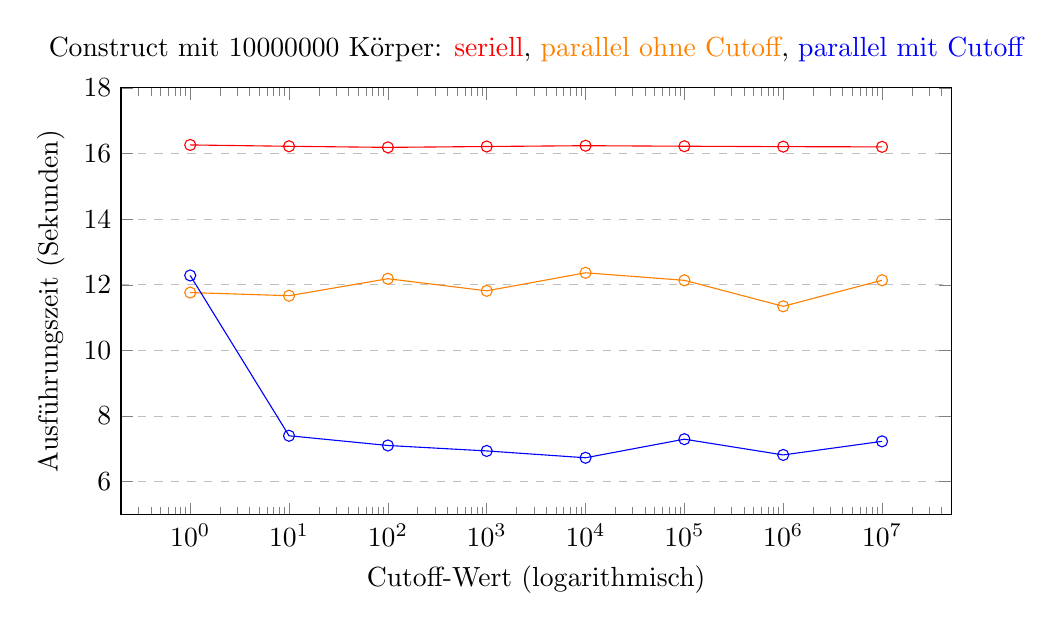
\begin{tikzpicture}
  \begin{axis}[
      xmode=log,
      width=\textwidth,
      height=7cm,
      title={Construct mit 10000000 Körper: \textcolor{red}{seriell}, \textcolor{orange}{parallel ohne Cutoff}, \textcolor{blue}{parallel mit Cutoff}},
      xlabel={Cutoff-Wert (logarithmisch)},
      ylabel={Ausführungszeit (Sekunden)},
      % xmin=0, xmax=100,
      % restrict y to domain=0:1000,
      % xtick={0,1,2,3,4,5,6,7,8,9},
      % ytick={0,20,40,60,80,100,120},
      % ymin=-3, ymax=20,
      % ytick={0, 5, 10, 15, 20},
      restrict y to domain=5:18,
      ymin=5, ymax=18,
      scaled ticks=false,
      % tick label style={/pgf/number format/fixed},
      legend pos=north west,
      ymajorgrids=true,
      grid style=dashed,
    ]

    \addplot[
      color=red,
      mark=o,
    ]
    coordinates {
        (1, 16.2612)
        (10, 16.2198)
        (100, 16.187)
        (1000, 16.2136)
        (10000, 16.2382)
        (100000, 16.2218)
        (1000000, 16.2092)
        (10000000, 16.2022)
      };

    \addplot[
      color=orange,
      mark=o,
    ]
    coordinates {
        (1, 11.7628)
        (10, 11.6672)
        (100, 12.1846)
        (1000, 11.8158)
        (10000, 12.366)
        (100000, 12.136)
        (1000000, 11.344)
        (10000000, 12.1392)
      };

    \addplot[
      color=blue,
      mark=o,
    ]
    coordinates {
        (1, 12.2842)
        (10, 7.4002)
        (100, 7.1038)
        (1000, 6.9376)
        (10000, 6.7296)
        (100000, 7.2956)
        (1000000, 6.8158)
        (10000000, 7.2294)
      };

  \end{axis}
\end{tikzpicture}

Wie in diesem Diagramm zu sehen ist, ist die parallele Funktion ohne ``Cutoff''-Wert 25\% schneller. Wenn der ``Cutoff''-Wert sehr niedrig eingestellt ist, gibt es keinen großen Unterschied, da die Funktion vollständig parallel ausgeführt wird, aber wenn dieser Wert erhöht wird, werden die kleineren Aufgaben seriell ausgeführt und die Funktion ist erheblich schneller. Um einen genaueren Wert zu finden, wurde dieser Wert zwischen 10 gleichen Werten für jedes Intervall im Bereich $10^3$ - $10^4$ und $10^4$ - $10^5$ getestet, da der schnellste Wert im logarithmischen Test $10^4$ war. Die nächsten Grafiken stellen die Laufzeit der Funktion für diese Wertebereiche dar.

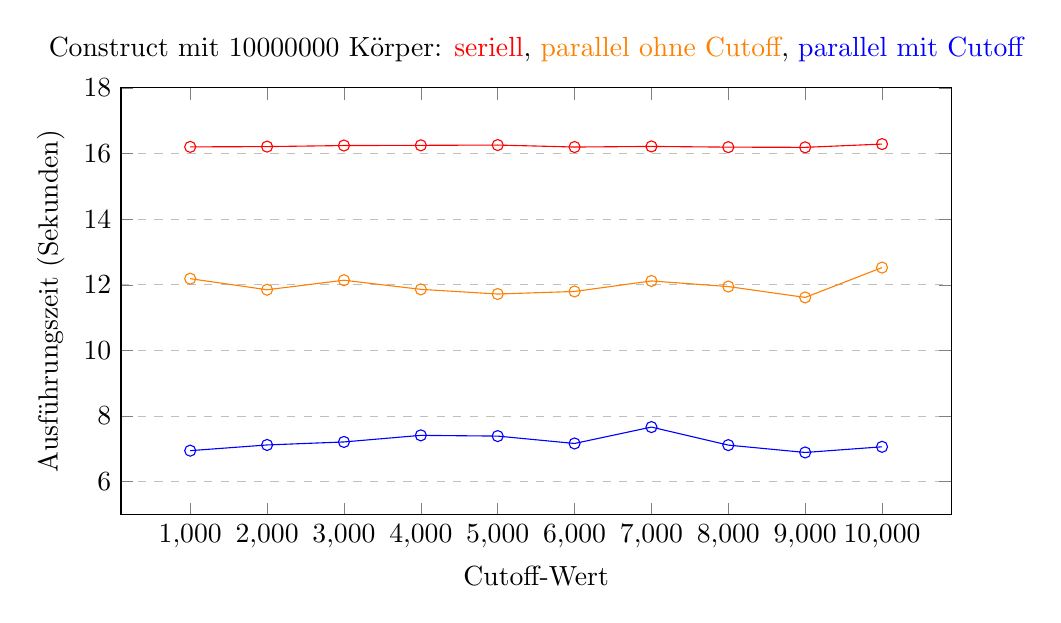
\begin{tikzpicture}
  \begin{axis}[
      width=\textwidth,
      height=7cm,
      title={Construct mit 10000000 Körper: \textcolor{red}{seriell}, \textcolor{orange}{parallel ohne Cutoff}, \textcolor{blue}{parallel mit Cutoff}},
      xlabel={Cutoff-Wert},
      ylabel={Ausführungszeit (Sekunden)},
      % xmin=0, xmax=100,
      % xtick={0,1,2,3,4,5,6,7,8,9},
      % ytick={0,20,40,60,80,100,120},
      restrict y to domain=5:18,
      ymin=5, ymax=18,
      % ytick={0, 5, 10, 15, 20},
      scaled ticks=false,
      % tick label style={/pgf/number format/fixed},
      legend pos=north west,
      ymajorgrids=true,
      grid style=dashed,
    ]

    \addplot[
      color=red,
      mark=o,
    ]
    coordinates {
        (1000, 16.202)
        (2000, 16.2104)
        (3000, 16.2428)
        (4000, 16.2492)
        (5000, 16.2578)
        (6000, 16.1974)
        (7000, 16.2158)
        (8000, 16.1944)
        (9000, 16.188)
        (10000, 16.2874)
      };

    \addplot[
      color=orange,
      mark=o,
    ]
    coordinates {
        (1000, 12.1862)
        (2000, 11.8488)
        (3000, 12.139)
        (4000, 11.8606)
        (5000, 11.7188)
        (6000, 11.797)
        (7000, 12.1168)
        (8000, 11.9458)
        (9000, 11.615)
        (10000, 12.5244)
      };

    \addplot[
      color=blue,
      mark=o,
    ]
    coordinates {
        (1000, 6.9462)
        (2000, 7.1196)
        (3000, 7.2114)
        (4000, 7.4122)
        (5000, 7.3896)
        (6000, 7.165)
        (7000, 7.6644)
        (8000, 7.1148)
        (9000, 6.891)
        (10000, 7.0632)
      };

  \end{axis}
\end{tikzpicture}

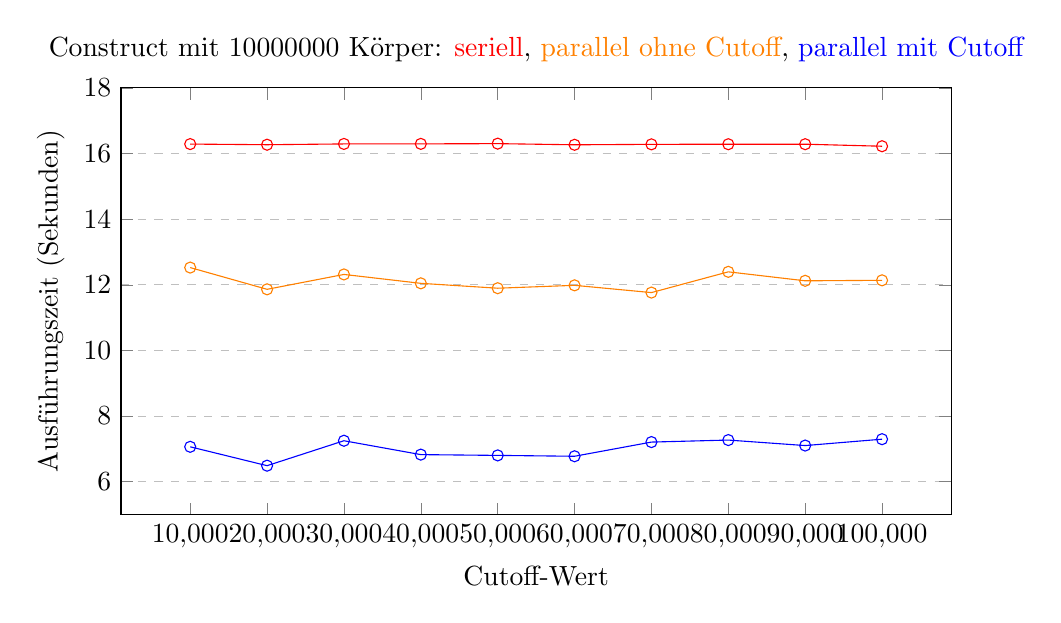
\begin{tikzpicture}
  \begin{axis}[
      width=\textwidth,
      height=7cm,
      title={Construct mit 10000000 Körper: \textcolor{red}{seriell}, \textcolor{orange}{parallel ohne Cutoff}, \textcolor{blue}{parallel mit Cutoff}},
      xlabel={Cutoff-Wert},
      ylabel={Ausführungszeit (Sekunden)},
      % xmin=0, xmax=100,
      % restrict y to domain=0:1000,
      % xtick={0,1,2,3,4,5,6,7,8,9},
      % ytick={0,20,40,60,80,100,120},
      % ymin=-3, ymax=20,
      % ytick={0, 5, 10, 15, 20},
      restrict y to domain=5:18,
      ymin=5, ymax=18,
      scaled ticks=false,
      tick label style={/pgf/number format/fixed},
      legend pos=north west,
      ymajorgrids=true,
      grid style=dashed,
    ]

    \addplot[
      color=red,
      mark=o,
    ]
    coordinates {
        (10000, 16.2874)
        (20000, 16.268)
        (30000, 16.2918)
        (40000, 16.2936)
        (50000, 16.3008)
        (60000, 16.2658)
        (70000, 16.2792)
        (80000, 16.283)
        (90000, 16.2838)
        (100000, 16.2218)

      };

    \addplot[
      color=orange,
      mark=o,
    ]
    coordinates {
        (10000, 12.5244)
        (20000, 11.862)
        (30000, 12.3154)
        (40000, 12.0444)
        (50000, 11.8958)
        (60000, 11.9834)
        (70000, 11.7624)
        (80000, 12.3946)
        (90000, 12.1214)
        (100000, 12.136)
      };

    \addplot[
      color=blue,
      mark=o,
    ]
    coordinates {
        (10000, 7.0632)
        (20000, 6.4882)
        (30000, 7.2482)
        (40000, 6.8254)
        (50000, 6.8016)
        (60000, 6.7752)
        (70000, 7.2074)
        (80000, 7.2688)
        (90000, 7.1014)
        (100000, 7.2956)

      };

  \end{axis}
\end{tikzpicture}

Das Ergebnis dieser Tests war, dass die schnellste Ausführungszeit erreicht wurde, wenn der ``Cutoff''-Wert auf 20000 gesetzt wurde. Mit einem Durchschnitt von 6488,2 Millisekunden war sie etwa 60\% schneller als die serielle Methode (durchschnittlich 16268 Millisekunden). Wurde die Funktion vollständig parallel ohne die ``Cutoff''-Werte ausgeführt, war sie nur etwa 30\% schneller als die serielle Methode (durchschnittlich 11862 Millisekunden).

\end{document}
